% Options for packages loaded elsewhere
\PassOptionsToPackage{unicode}{hyperref}
\PassOptionsToPackage{hyphens}{url}
\documentclass[
  11pt,
]{article}
\usepackage{xcolor}
\usepackage[margin=22mm]{geometry}
\usepackage{amsmath,amssymb}
\setcounter{secnumdepth}{-\maxdimen} % remove section numbering
\usepackage{iftex}
\ifPDFTeX
  \usepackage[T1]{fontenc}
  \usepackage[utf8]{inputenc}
  \usepackage{textcomp} % provide euro and other symbols
\else % if luatex or xetex
  \usepackage{unicode-math} % this also loads fontspec
  \defaultfontfeatures{Scale=MatchLowercase}
  \defaultfontfeatures[\rmfamily]{Ligatures=TeX,Scale=1}
\fi
\usepackage{lmodern}
\ifPDFTeX\else
  % xetex/luatex font selection
\fi
% Use upquote if available, for straight quotes in verbatim environments
\IfFileExists{upquote.sty}{\usepackage{upquote}}{}
\IfFileExists{microtype.sty}{% use microtype if available
  \usepackage[]{microtype}
  \UseMicrotypeSet[protrusion]{basicmath} % disable protrusion for tt fonts
}{}
\makeatletter
\@ifundefined{KOMAClassName}{% if non-KOMA class
  \IfFileExists{parskip.sty}{%
    \usepackage{parskip}
  }{% else
    \setlength{\parindent}{0pt}
    \setlength{\parskip}{6pt plus 2pt minus 1pt}}
}{% if KOMA class
  \KOMAoptions{parskip=half}}
\makeatother
\usepackage{graphicx}
\makeatletter
\newsavebox\pandoc@box
\newcommand*\pandocbounded[1]{% scales image to fit in text height/width
  \sbox\pandoc@box{#1}%
  \Gscale@div\@tempa{\textheight}{\dimexpr\ht\pandoc@box+\dp\pandoc@box\relax}%
  \Gscale@div\@tempb{\linewidth}{\wd\pandoc@box}%
  \ifdim\@tempb\p@<\@tempa\p@\let\@tempa\@tempb\fi% select the smaller of both
  \ifdim\@tempa\p@<\p@\scalebox{\@tempa}{\usebox\pandoc@box}%
  \else\usebox{\pandoc@box}%
  \fi%
}
% Set default figure placement to htbp
\def\fps@figure{htbp}
\makeatother
\setlength{\emergencystretch}{3em} % prevent overfull lines
\providecommand{\tightlist}{%
  \setlength{\itemsep}{0pt}\setlength{\parskip}{0pt}}
\usepackage{bookmark}
\IfFileExists{xurl.sty}{\usepackage{xurl}}{} % add URL line breaks if available
\urlstyle{same}
\hypersetup{
  hidelinks,
  pdfcreator={LaTeX via pandoc}}

\author{}
\date{}

\ExplSyntaxOn
\cs_new:Npn \ReaderIfNativeAnchorTF #1 { \exp_args:Nx \str_if_in:nnTF {#1} {section*.} }
\ExplSyntaxOff
\makeatletter
\let\ReaderOriginalAnchorStart\hyper@anchorstart
\let\ReaderOriginalAnchorEnd\hyper@anchorend
\let\ReaderPendingAliases\@empty
\def\ReaderArmAliases#1{\gdef\ReaderPendingAliases{#1}}
\def\hyper@anchorstart#1{\ReaderIfNativeAnchorTF{#1}{\ReaderPendingAliases\global\let\ReaderPendingAliases\@empty}{}\ReaderOriginalAnchorStart{#1}}
\makeatother
\begin{document}

\section{Boundary wave fronts for elliptic
systems}\label{boundary-wave-fronts-for-elliptic-systems}

For an elliptic boundary problem, a boundary singularity of the solution
is exactly a singularity of the interior forcing or of one of the
boundary measurements. Proving that equality requires two different
regularity gains. Before traces are available, the normal equation moves
one unit from the tangential weight into the total-frequency weight.
Once the trace threshold is reached, the generalized boundary parametrix
raises total-frequency regularity while keeping the tangential weight
fixed.

This lesson proves the equality with all normal powers and both Sobolev
exponents visible. It then defines the local characteristic set for a
differential boundary problem, deletes only redundant boundary output
coordinates, completes the coefficients outside a selected tangential
cone, and proves the local microlocal inclusion. The final section
separates two doubling-index conventions by exact block-sum algebra.

Named prerequisites are \href{global-boundary-calculus.pdf}{Global
boundary calculus on the compressed cotangent bundle},
\href{mixed-sobolev-mapping.pdf}{Sobolev mapping with normal and
tangential weights}, and \href{generalized-collar-fredholm.pdf}{Fredholm
boundary problems with first-order Calderón defects}. The proof uses
their tangential tester, two-weight mapping theorem, trace theorem, and
local generalized parametrix with the hypotheses stated there.

Throughout, \(D=-i\partial\). Matrix factors keep their displayed order.
Every wave-front statement is local in a product collar and is invariant
under the bundle and compressed-cotangent coordinate maps proved in the
first named prerequisite.

\begin{figure}
\centering
\pandocbounded{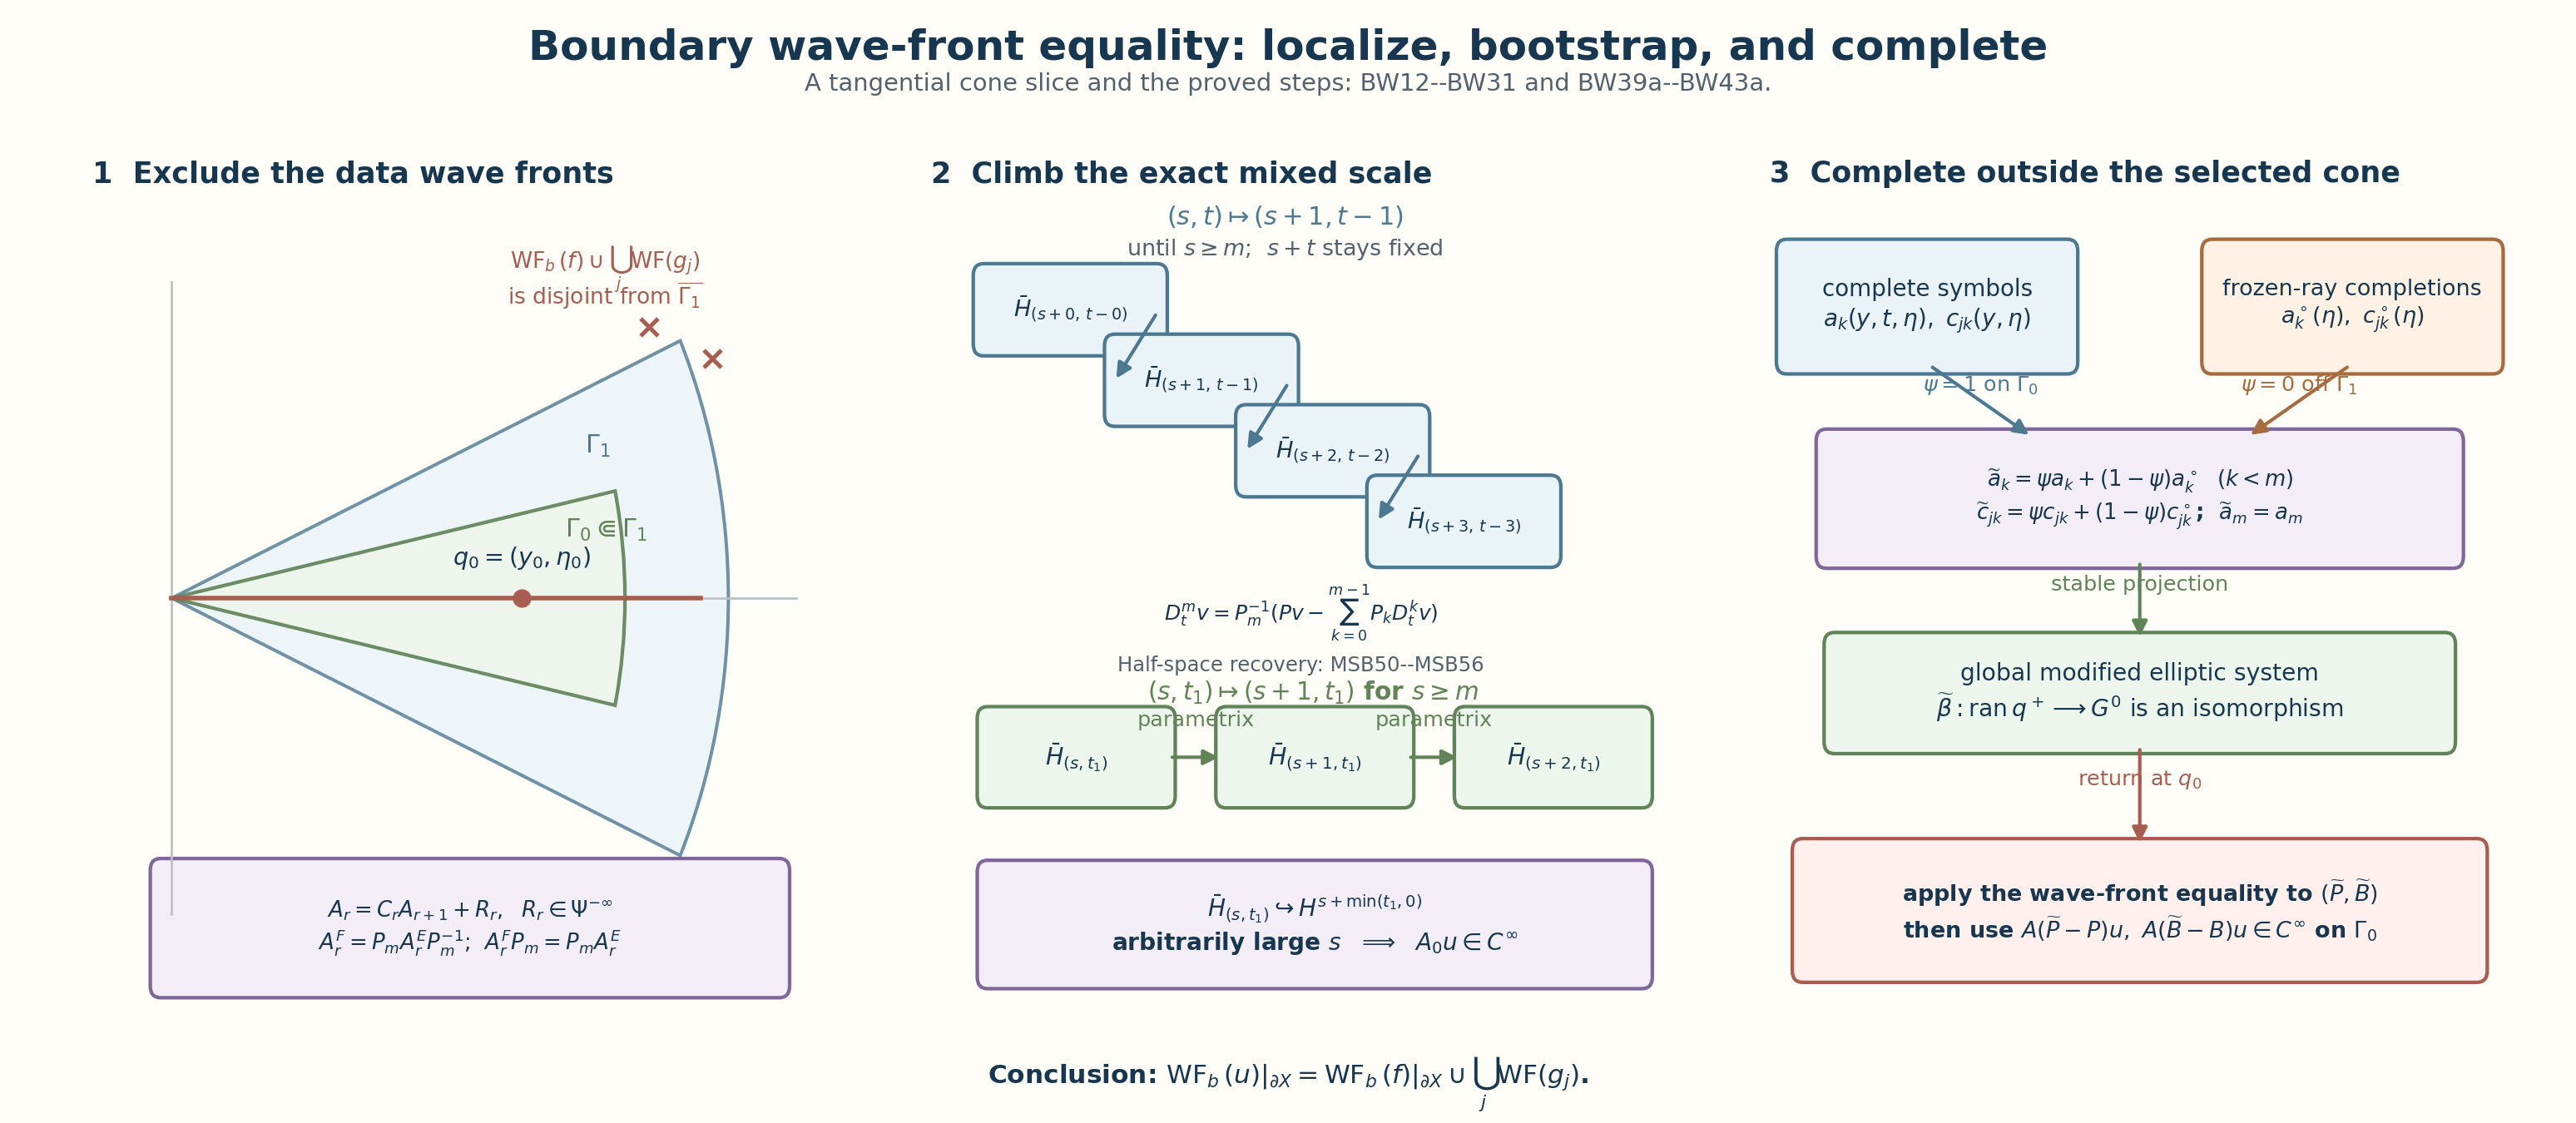
\includegraphics[keepaspectratio,alt={Nested tangential cones, the two-stage Sobolev bootstrap, and the local elliptic completion.}]{../figures/boundary_wavefront_bootstrap.png}}
\caption{Nested tangential cones, the two-stage Sobolev bootstrap, and
the local elliptic completion.}
\end{figure}

\ReaderArmAliases{\ReaderOriginalAnchorStart{AN03-BWF-001}\ReaderOriginalAnchorEnd\begingroup\expandafter\def\csname @currentHref\endcsname{AN03-BWF-001}\label{AN03-BWF-001}\endgroup\ReaderOriginalAnchorStart{1-the-boundary-class-and-the-normalized-system}\ReaderOriginalAnchorEnd\begingroup\expandafter\def\csname @currentHref\endcsname{1-the-boundary-class-and-the-normalized-system}\label{1-the-boundary-class-and-the-normalized-system}\endgroup\ReaderOriginalAnchorStart{1-the-boundary-class-and-the-original-system}\ReaderOriginalAnchorEnd\begingroup\expandafter\def\csname @currentHref\endcsname{1-the-boundary-class-and-the-original-system}\label{1-the-boundary-class-and-the-original-system}\endgroup}
\subsection{1. The boundary class and the original
system}\label{the-boundary-class-and-the-original-system}

Let \(\mathcal A(X)\) and \(\mathcal A'(X)\) be the conormal test and
dual classes from \href{global-boundary-calculus.pdf}{Global boundary
calculus on the compressed cotangent bundle}. Embed
\(T^*\partial X\setminus0\) in the boundary of the compressed cotangent
bundle by giving it zero compressed normal component. The
noncharacteristic extension class is

\[
 \mathcal N(X)=\{u\in\mathcal A'(X):
 \operatorname{WF}_b(u)|_{\partial X}
 \subset T^*\partial X\setminus0\}.
 \tag{BW1}
\]

Work in a collar \(Y\times[0,\varepsilon)_t\). Keep the original
generalized elliptic operator \(P:E\to F\), its invertible leading
normal bundle map \(P_m:E\to F\), and the boundary rows in the exact
form

\[
 \begin{aligned}
 P&=\sum_{k=0}^{m}P_k(t)D_t^k,
       &P_k(t)&\in\Psi_{\mathrm{tan}}^{m-k}(Y;E,F),\\
 P_m(t)&\text{ is multiplication by an invertible bundle map},\\
 B_j&=\sum_{k=0}^{m-1}B_{jk}\gamma_k,
       &B_{jk}&\in\Psi^{m_j-k}(Y;E,G_j),
 \qquad \gamma_k u=(D_t^ku)|_{t=0}.
 \end{aligned}
 \tag{BW2}
\]

No identification of \(E\) with \(F\) is implicit in this formula. The
input and output localizers below are related by the exact bundle
conjugation \(A^F=P_mA^EP_m^{-1}\); thus \(A^FP_m=P_mA^E\), with every
factor and domain retained. Assume the generalized principal polynomial
is elliptic and the principal boundary map is an isomorphism on its
stable Cauchy bundle. Let

\[
 u,f\in\mathcal N(X),\qquad Pu=f\text{ on }X^\circ,
 \qquad B_ju=g_j\in\mathcal D'(Y,G_j).
 \tag{BW3}
\]

The global theorem below is first proved for a compactly supported
collar localization. Proper supports and a finite collar partition then
give the stated manifold result.

\ReaderArmAliases{\ReaderOriginalAnchorStart{AN03-BWF-002}\ReaderOriginalAnchorEnd\begingroup\expandafter\def\csname @currentHref\endcsname{AN03-BWF-002}\label{AN03-BWF-002}\endgroup\ReaderOriginalAnchorStart{2-the-data-cannot-have-more-boundary-singularities-than-the-solution}\ReaderOriginalAnchorEnd\begingroup\expandafter\def\csname @currentHref\endcsname{2-the-data-cannot-have-more-boundary-singularities-than-the-solution}\label{2-the-data-cannot-have-more-boundary-singularities-than-the-solution}\endgroup}
\subsection{2. The data cannot have more boundary singularities than the
solution}\label{the-data-cannot-have-more-boundary-singularities-than-the-solution}

Fix \(q\notin\operatorname{WF}_b(u)|_Y\). Choose scalar tangential
testers \(A_0^E,A_1^E\), acting by scalar symbols in input bundle
frames, such that \(A_0^E\) is elliptic at \(q\), \(A_1^E\) has identity
symbol on a neighborhood of the microsupport of \(A_0^E\), and
\(A_0^Eu,A_1^Eu\) are smooth. Set \(A_0^F=P_mA_0^EP_m^{-1}\). Take both
symbols independent of \(t\) next to the boundary. Then

\[
 A_0^FPu=P A_0^Eu+
       (A_0^FP-PA_0^E)A_1^Eu+
       \sum_{l=0}^{m-1}R_lD_t^lu,
 \qquad R_l\in\Psi^{-\infty}_{\mathrm{tan}}(E,F).
 \tag{BW3a}
\]

microlocally at \(q\). Indeed, expand the commutator by normal power.
Its highest coefficient vanishes because \(A_0^FP_m=P_mA_0^E\); the
lower coefficients and all normal derivatives are given explicitly in
(BW15). Each has microsupport in that of \(A_0^E\), so the identity
region of \(A_1^E\) inserts \(A_1^E\); the remainder is tangentially
smoothing. The first two terms on the right of (BW3a) are smooth because
\(A_0^Eu\) and \(A_1^Eu\) are smooth. Each retained normal jet has the
ordinary-normal pseudolocal property proved in GW12. The remainders have
no nonzero tangential boundary covector, and the class \(\mathcal N(X)\)
excludes a residual zero-tangential boundary wave-front point. This
proves the required pseudolocal statement with the ordinary normal
derivatives retained:

\[
 \operatorname{WF}_b(f)|_Y
 =\operatorname{WF}_b(Pu)|_Y
 \subset\operatorname{WF}_b(u)|_Y.
 \tag{BW4}
\]

Every interior normal jet has the same tangential implication. To see
this without treating \(D_t\) as a compressed operator, fix
\(q=(y,\eta)\notin\operatorname{WF}_b(u)|_Y\). The tangential tester
theorem in the global boundary calculus lesson supplies a properly
supported \(A=a(y,t,D_y)\), elliptic at \(q\), for which \(Au\) is
smooth. In its construction take \(a\) independent of \(t\) near
\(t=0\). Then for every \(k\geq0\), exactly

\[
 a(y,0,D_y)\gamma_ku=\gamma_k(Au).
 \tag{BW5}
\]

The right side is smooth and the left boundary operator is elliptic at
\(q\). Its ordinary tangential parametrix proves

\[
 \operatorname{WF}(\gamma_ku)
 \subset\operatorname{WF}_b(u)|_Y
 \qquad(k\geq0).
 \tag{BW6}
\]

Tangential pseudolocality of every \(B_{jk}\), with its actual bundle
map, now gives

\[
 \operatorname{WF}(g_j)
 \subset\bigcup_{k<m}\operatorname{WF}(\gamma_ku)
 \subset\operatorname{WF}_b(u)|_Y.
 \tag{BW7}
\]

Thus the forcing and all boundary data give the first inclusion in the
desired equality.

\ReaderArmAliases{\ReaderOriginalAnchorStart{AN03-BWF-003}\ReaderOriginalAnchorEnd\begingroup\expandafter\def\csname @currentHref\endcsname{AN03-BWF-003}\label{AN03-BWF-003}\endgroup\ReaderOriginalAnchorStart{3-the-exact-mixed-normal-recovery-inequality}\ReaderOriginalAnchorEnd\begingroup\expandafter\def\csname @currentHref\endcsname{3-the-exact-mixed-normal-recovery-inequality}\label{3-the-exact-mixed-normal-recovery-inequality}\endgroup}
\subsection{3. The exact mixed normal-recovery
inequality}\label{the-exact-mixed-normal-recovery-inequality}

In a collar chart write

\[
 R_0(\xi',\xi_n)=(1+|\xi'|^2+\xi_n^2)^{1/2},
 \qquad T_0(\xi')=(1+|\xi'|^2)^{1/2},
 \tag{BW8}
\]

and use the two-weight norm with weight \(R_0^sT_0^t\). The elementary
inequality that controls the preliminary bootstrap is, for
\(0\leq j\leq m\),

\[
 |\xi_n|^jR_0^{s-j+1}T_0^{t-1}
 \leq 2^{m/2}
 \left(R_0^sT_0^t
 +|\xi_n|^mR_0^{s-m+1}T_0^{t-1}\right).
 \tag{BW9}
\]

On \(|\xi_n|\leq T_0\), divide the left side by the first term. The
quotient is \(R_0T_0^{-1}(|\xi_n|/R_0)^j\leq\sqrt2\). On
\(|\xi_n|\geq T_0\), divide by the second term. The quotient is
\((R_0/|\xi_n|)^{m-j}\leq2^{(m-j)/2}\). These two regions prove (BW9),
including \(j=0\) and \(j=m\).

For whole-space inputs, Plancherel applies directly to (BW9). For the
actual restriction spaces we instead use the complete half-space
argument MSB50--MSB56 in \href{mixed-sobolev-mapping.pdf}{Mixed symbols
on every real two-parameter Sobolev scale}. It constructs the inverse of
\(D_t+i\Lambda\), proves uniqueness of its tempered half-space solution,
and retains every term of \((D_t+i\Lambda)^mv\). It gives the exact
normal-recovery implication

\[
 v\in\bar H_{(s,t)},\quad
 D_t^mv\in\bar H_{(s-m+1,t-1)}
 \Longrightarrow
 D_t^jv\in\bar H_{(s-j+1,t-1)}
 \quad(0\leq j\leq m).
 \tag{BW10}
\]

No interpolation endpoint or integer condition on \(s,t\) is used.

We shall also use the exact mixed embedding behind every lower normal
term. If \(0\leq k<m\), a tangential operator of order \(m-k\) maps
\(D_t^kv\), initially in \(\bar H_{(s-k,t)}\), into
\(\bar H_{(s-k,t-m+k)}\). Since \(T_0\leq R_0\),

\[
 \bar H_{(s-k,t-m+k)}
 \hookrightarrow\bar H_{(s-m+1,t-1)}.
 \tag{BW11}
\]

The quotient of the target weight by the source weight is
\((T_0/R_0)^{m-k-1}\leq1\). This keeps both weights and every normal
power visible.

\ReaderArmAliases{\ReaderOriginalAnchorStart{AN03-BWF-004}\ReaderOriginalAnchorEnd\begingroup\expandafter\def\csname @currentHref\endcsname{AN03-BWF-004}\label{AN03-BWF-004}\endgroup\ReaderOriginalAnchorStart{4-admissible-tangential-localizers-and-their-commutators}\ReaderOriginalAnchorEnd\begingroup\expandafter\def\csname @currentHref\endcsname{4-admissible-tangential-localizers-and-their-commutators}\label{4-admissible-tangential-localizers-and-their-commutators}\endgroup}
\subsection{4. Admissible tangential localizers and their
commutators}\label{admissible-tangential-localizers-and-their-commutators}

Fix \(q_0=(y_0,\eta_0)\in T^*Y\setminus0\) outside the boundary wave
fronts of \(f\) and every \(g_j\). Choose nested base-cone neighborhoods

\[
 V_0\times\Gamma_0\Subset V_1\times\Gamma_1
 \Subset\cdots\Subset V_N\times\Gamma_N
 \tag{BW12}
\]

whose largest closure misses those data wave fronts. Because
\(u,f\in\mathcal N\), the collar may also be chosen so that no relevant
boundary wave-front point has \(\xi'=0\). Let \(A_r^E\) be a scalar,
properly supported, order-zero tangential operator in the input bundle,
supported in \(V_{r+1}\times\Gamma_{r+1}\), elliptic and equal to the
identity symbol on \(V_r\times\Gamma_r\), with a normal cutoff in the
collar. Choose the normal cutoffs nested as well: each outer cutoff is
one on a neighborhood of the support of the inner cutoff and all of its
normal derivatives. Finitely many such cutoffs exist between two fixed
collar neighborhoods by the smooth cutoff construction. Use its scalar
boundary symbol on each \(G_j\) to define \(A_r^{G_j}\), and define
\(A_r^F=P_mA_r^EP_m^{-1}\). Multiplication by the smooth invertible
bundle maps preserves its order, microsupport and scalar principal
symbol. For brevity, \(A_r\) on an input \(u\) means \(A_r^E\). Then

\[
 A_r^Ff\in C^\infty,\qquad A_r^{G_j}g_j\in C^\infty,
 \qquad A_r=C_rA_{r+1}+R_r,\quad R_r\in\Psi^{-\infty}
 \tag{BW13}
\]

microlocally on \(V_r\times\Gamma_r\). The last identity follows by an
ordinary tangential parametrix for \(A_{r+1}\) on the microsupport of
\(A_r\); it is the precise meaning of an admissible nested cutoff.

With the domain-correct commutator
\(\mathcal C_r=PA_r^E-A_r^FP:E\to F\), the original top coefficient in
(BW2) gives

\[
 \mathcal C_r=\sum_{k=0}^{m-1}C_{rk}D_t^k,
 \qquad C_{rk}\in\Psi_{\mathrm{tan}}^{m-k-1}.
 \tag{BW14}
\]

Here is the complete order check. For a coefficient \(P_lD_t^l\),

\[
 P_lD_t^lA_r^E-A_r^FP_lD_t^l
 =(P_lA_r^E-A_r^FP_l)D_t^l
 +P_l\sum_{h=0}^{l-1}\binom lh
       (D_t^{\,l-h}A_r^E)D_t^h.
 \tag{BW15}
\]

Because \(A_r^E\) and \(A_r^F\) have the same scalar principal symbol,
the leading symbols of \(P_lA_r^E\) and \(A_r^FP_l\) agree as maps
\(E\to F\); therefore the first commutator coefficient drops by one
tangential order and has order \((m-l)-1\). In the summand with normal
power \(h<l\), the coefficient has order \(m-l\leq m-h-1\). When
\(l=m\), the first term vanishes because \(P_mA_r^E=A_r^FP_m\) exactly,
with the original \(P_m\) retained. This proves (BW14), including every
binomial factor and normal derivative of the localizer.

For the boundary rows put \(A_{r,a}^E=(D_t^aA_r^E)|_{t=0}\). Each normal
derivative of this tangential family has order zero. The full boundary
calculation gives

\[
 \begin{aligned}
 \mathcal C_{rj}&=B_jA_r^E-A_r^{G_j}B_j\\
 &=\sum_{k=0}^{m-1}
       (B_{jk}A_{r,0}^E-A_r^{G_j}B_{jk})\gamma_k\\
 &\quad+\sum_{k=0}^{m-1}\sum_{a=1}^{k}
       \binom ka B_{jk}A_{r,a}^E\gamma_{k-a}\\
 &=\sum_{k=0}^{m-1}C_{rjk}\gamma_k,\qquad
       C_{rjk}\in\Psi^{m_j-k-1}(E,G_j).
 \end{aligned}
 \tag{BW16}
\]

The first sum drops an order because the two localizers have the same
scalar principal symbol. In the second sum a coefficient acts on jet
\(l=k-a\) and has order \(m_j-k=m_j-l-a\leq m_j-l-1\). This proves the
required bound with all binomial factors, normal derivatives and matrix
orders retained. All coefficients in (BW14) and (BW16) have microsupport
where \(A_{r+1}\) is elliptic. Thus (BW13) inserts \(A_{r+1}u\) after
each coefficient, modulo a smooth remainder, without changing the
displayed orders.

Finally, a compactly supported distribution has finite order. Its
Fourier transform grows by a fixed power of \(R_0\), so for some real
\(s_0,t_0\), and hence for the outermost localizer,

\[
 A_Nu\in\bar H_{(s_0,t_0)}.
 \tag{BW17}
\]

This is only the starting level; no unproved regularity is inserted.

\ReaderArmAliases{\ReaderOriginalAnchorStart{AN03-BWF-005}\ReaderOriginalAnchorEnd\begingroup\expandafter\def\csname @currentHref\endcsname{AN03-BWF-005}\label{AN03-BWF-005}\endgroup\ReaderOriginalAnchorStart{5-reaching-the-trace-range-while-preserving-the-total-weight}\ReaderOriginalAnchorEnd\begingroup\expandafter\def\csname @currentHref\endcsname{5-reaching-the-trace-range-while-preserving-the-total-weight}\label{5-reaching-the-trace-range-while-preserving-the-total-weight}\endgroup}
\subsection{5. Reaching the trace range while preserving the total
weight}\label{reaching-the-trace-range-while-preserving-the-total-weight}

Assume \(A_{r+1}u\in\bar H_{(s,t)}\) and set \(v=A_ru\). Equations
(BW13)--(BW16) and the mixed mapping theorem give

\[
 Pv=A_r^Ff+\mathcal C_ru\in\bar H_{(s-m+1,t)}.
 \tag{BW18}
\]

Every lower term \(P_kD_t^kv\) belongs to the source space in (BW11),
hence to \(\bar H_{(s-m+1,t-1)}\). The right side of (BW18) embeds in
that same space. Solving the original equation for its highest normal
derivative gives

\[
 D_t^mv=P_m^{-1}\left(Pv-\sum_{k<m}P_kD_t^kv\right)
 \in\bar H_{(s-m+1,t-1)}.
 \tag{BW19}
\]

The multiplication map \(P_m^{-1}:F\to E\) is bounded on these localized
mixed spaces by the order-zero mapping theorem. Thus the membership in
(BW19) is proved with every original \(P_k\) and \(P_m\) present. The
recovery implication (BW10) now yields the one-step gain

\[
 A_ru=v\in\bar H_{(s+1,t-1)}.
 \tag{BW20}
\]

The total exponent \(s+t\) is unchanged. Starting with (BW17) and using
a finite nested family, repeat (BW20) until the first exponent is at
least \(m\):

\[
 A_ru\in\bar H_{(s_1,t_1)},\qquad s_1\geq m,
 \qquad s_1+t_1=s_0+t_0.
 \tag{BW21}
\]

The number of steps is finite even when \(s_0\) is not an integer.

\ReaderArmAliases{\ReaderOriginalAnchorStart{AN03-BWF-006}\ReaderOriginalAnchorEnd\begingroup\expandafter\def\csname @currentHref\endcsname{AN03-BWF-006}\label{AN03-BWF-006}\endgroup\ReaderOriginalAnchorStart{6-the-boundary-parametrix-then-gains-normal-order-at-fixed-tangential-weight}\ReaderOriginalAnchorEnd\begingroup\expandafter\def\csname @currentHref\endcsname{6-the-boundary-parametrix-then-gains-normal-order-at-fixed-tangential-weight}\label{6-the-boundary-parametrix-then-gains-normal-order-at-fixed-tangential-weight}\endgroup}
\subsection{6. The boundary parametrix then gains normal order at fixed
tangential
weight}\label{the-boundary-parametrix-then-gains-normal-order-at-fixed-tangential-weight}

Suppose now that \(A_{r+1}u\in\bar H_{(s,t)}\) with \(s\geq m\), and
again set \(v=A_ru\). The mixed trace theorem gives

\[
 \gamma_kv\in H^{s+t-k-1/2}(Y,E)
 \qquad(0\leq k<m).
 \tag{BW22}
\]

Use the boundary equation, with the commutator convention matching
(BW16):

\[
 B_jv=A_r^{G_j}g_j+\mathcal C_{rj}u.
 \tag{BW23}
\]

The first term is smooth. Each term of the second has order \(m_j-k-1\)
on a trace of order \(s+t-k-1/2\). Therefore

\[
 B_jv\in H^{s+t-m_j+1/2}(Y,G_j).
 \tag{BW24}
\]

Together with (BW18), these are exactly the data spaces for one more
first mixed exponent at fixed \(t\):

\[
 Pv\in\bar H_{((s+1)-m,t)},\qquad
 B_jv\in H^{(s+1)+t-m_j-1/2}.
 \tag{BW25}
\]

Apply the local generalized parametrix proved in
\href{generalized-collar-fredholm.pdf}{Fredholm boundary problems with
first-order Calderón defects}. Its terms have the unchanged mappings

\[
 \begin{aligned}
 V&:\bar H_{((s+1)-m,t)}\longrightarrow\bar H_{(s+1,t)},\\
 KS&:\bigoplus_jH^{(s+1)+t-m_j-1/2}
       \longrightarrow\bar H_{(s+1,t)},\\
 \mathscr K&:\bar H_{(s,t)}\longrightarrow\bar H_{(s+1,t)}.
 \end{aligned}
 \tag{BW26}
\]

The localized identity \(v=\mathscr L(Pv,Bv)+\mathscr Kv\) and
(BW25)--(BW26) prove

\[
 A_ru\in\bar H_{(s+1,t)}\qquad(s\geq m).
 \tag{BW27}
\]

For every requested \(M\), take a nested family long enough to combine
(BW20) up to \(s\geq m\) with \(M\) uses of (BW27). The innermost
localizer is fixed and elliptic at \(q_0\). Hence it maps \(u\) into
\(\bar H_{(s,t_1)}\) for arbitrarily large \(s\). Since \(T_0\leq R_0\),
for fixed \(t_1\)

\[
 \bar H_{(s,t_1)}\hookrightarrow H^{s+\min(t_1,0)},
 \tag{BW28}
\]

so local Sobolev embedding at arbitrarily large order proves

\[
 A_0u\in C^\infty(X).
 \tag{BW29}
\]

By the tangential tester theorem,
\(q_0\notin\operatorname{WF}_b(u)|_Y\). This closes every
normal-derivative, boundary-commutator, and nonintegral-exponent step in
the reverse inclusion.

\ReaderArmAliases{\ReaderOriginalAnchorStart{AN03-BWF-007}\ReaderOriginalAnchorEnd\begingroup\expandafter\def\csname @currentHref\endcsname{AN03-BWF-007}\label{AN03-BWF-007}\endgroup\ReaderOriginalAnchorStart{7-boundary-wave-front-equality-for-a-generalized-elliptic-problem}\ReaderOriginalAnchorEnd\begingroup\expandafter\def\csname @currentHref\endcsname{7-boundary-wave-front-equality-for-a-generalized-elliptic-problem}\label{7-boundary-wave-front-equality-for-a-generalized-elliptic-problem}\endgroup}
\subsection{7. Boundary wave-front equality for a generalized elliptic
problem}\label{boundary-wave-front-equality-for-a-generalized-elliptic-problem}

The argument in Sections 4--6 applies at every covector outside the
forcing and boundary-data wave fronts. It proves

\[
 \operatorname{WF}_b(u)|_Y
 \subset\operatorname{WF}_b(f)|_Y
      \cup\bigcup_j\operatorname{WF}(g_j).
 \tag{BW30}
\]

Combine this with (BW4) and (BW7):

\[
 \boxed{\operatorname{WF}_b(u)|_{\partial X}
 =\operatorname{WF}_b(f)|_{\partial X}
      \cup\bigcup_j\operatorname{WF}(g_j).}
 \tag{BW31}
\]

This proves the boundary wave-front equality with every normal and
tangential exponent displayed. The class \(\mathcal N(X)\) is essential:
it supplies the tangential boundary hyperplane in (BW1), the intrinsic
jets in (BW5), and the tangential tester theorem. Nothing here asserts
(BW31) for an arbitrary boundary-supported distribution.

\ReaderArmAliases{\ReaderOriginalAnchorStart{AN03-BWF-008}\ReaderOriginalAnchorEnd\begingroup\expandafter\def\csname @currentHref\endcsname{AN03-BWF-008}\label{AN03-BWF-008}\endgroup\ReaderOriginalAnchorStart{8-the-local-characteristic-set-for-a-differential-boundary-problem}\ReaderOriginalAnchorEnd\begingroup\expandafter\def\csname @currentHref\endcsname{8-the-local-characteristic-set-for-a-differential-boundary-problem}\label{8-the-local-characteristic-set-for-a-differential-boundary-problem}\endgroup}
\subsection{8. The local characteristic set for a differential boundary
problem}\label{the-local-characteristic-set-for-a-differential-boundary-problem}

Now let \(P:C^\infty(X,E)\to C^\infty(X,F)\) be an arbitrary order-\(m\)
differential operator between equal-rank complex bundles, with
noncharacteristic boundary. In a boundary chart its full homogeneous
principal polynomial is

\[
 \mathfrak p(y,\eta,\tau)
   =\sum_{k=0}^m p_k(y,\eta)\tau^k,
 \qquad p_k(y,\lambda\eta)=\lambda^{m-k}p_k(y,\eta).
 \tag{BW32}
\]

For \((y,\eta)\in T^*Y\setminus0\), let \(\mathscr M^+_{y,\eta}\) be the
finite-dimensional space of bounded solutions on \(t\geq0\) of

\[
 \mathfrak p(y,\eta,D_t)v(t)=0.
 \tag{BW33}
\]

This definition includes polynomial factors multiplying exponentials
when a normal root is multiple. Let the principal boundary map be

\[
 \beta_{y,\eta}:\mathscr M^+_{y,\eta}\longrightarrow
       \bigoplus_j(G_j)_y,\qquad
 v\longmapsto\bigl(b_j(y,\eta,D_t)v|_{t=0}\bigr)_j.
 \tag{BW34}
\]

The exact boundary characteristic set is

\[
 \operatorname{Char}(P;B)=
 \left\{(y,\eta):
 \begin{array}{l}
 \mathfrak p(y,\eta,\tau)\text{ is singular for some }\tau\in\mathbb R,
 \text{ or}\\
 \beta_{y,\eta}\text{ is not injective}
 \end{array}\right\}.
 \tag{BW35}
\]

The definition uses injectivity. Surjectivity is neither inserted nor
needed when the original boundary list contains redundant equations.

\ReaderArmAliases{\ReaderOriginalAnchorStart{AN03-BWF-009}\ReaderOriginalAnchorEnd\begingroup\expandafter\def\csname @currentHref\endcsname{AN03-BWF-009}\label{AN03-BWF-009}\endgroup\ReaderOriginalAnchorStart{9-completing-the-system-outside-a-narrow-tangential-cone}\ReaderOriginalAnchorEnd\begingroup\expandafter\def\csname @currentHref\endcsname{9-completing-the-system-outside-a-narrow-tangential-cone}\label{9-completing-the-system-outside-a-narrow-tangential-cone}\endgroup}
\subsection{9. Completing the system outside a narrow tangential
cone}\label{completing-the-system-outside-a-narrow-tangential-cone}

Fix \(q_0=(y_0,\eta_0)\notin\operatorname{Char}(P;B)\). Put
\(d=\dim\mathscr M^+_{q_0}\). In local frames the matrix of
\(\beta_{q_0}\) has column rank \(d\), so some \(d\times d\) minor is
nonzero. Retain exactly those \(d\) output components. Their boundary
map

\[
 \beta^0_{q_0}:\mathscr M^+_{q_0}\longrightarrow G^0_{q_0}
 \tag{BW36}
\]

is an isomorphism. This is a deletion of redundant local output
coordinates, not an alteration of the bounded solution space. The
discarded equations remain valid data equations but are not needed for
the regularity estimate.

Choose conic neighborhoods \(\Gamma_0\Subset\Gamma_1\) of the ray
\(\mathbb R_+\eta_0\), and a smooth degree-zero function \(\psi\) for
\(|\eta|\geq1\), equal to one on \(\Gamma_0\) and supported in
\(\Gamma_1\). Write

\[
 \eta^\circ(\eta)=\frac{|\eta|}{|\eta_0|}\eta_0.
 \tag{BW37}
\]

Write \(a_k(y,t,\eta)\) for a complete classical tangential symbol of
the coefficient of \(D_t^k\) in \(P\), and write \(c_{jk}(y,\eta)\) for
a complete symbol of the retained coefficient of \(\gamma_k\) in
\(B_j\). Their leading homogeneous terms are the coefficients \(p_k\)
and \(b_{jk}\) used in the principal polynomial and principal boundary
map. This distinction matters below: extending only \(p_k\) and
\(b_{jk}\) would leave the lower-order operator terms uncontrolled.

Retain the original leading normal coefficient. For \(k<m\) set

\[
 \widetilde p_k(y,t,\eta)
 =\psi(\eta)p_k(y,t,\eta)
 +(1-\psi(\eta))p_k(y_0,0,\eta^\circ(\eta)),
 \qquad \widetilde p_m=p_m(y,t).
 \tag{BW38}
\]

At bounded \(|\eta|\), join these formulas by a smooth cutoff; that
changes only low tangential frequencies. For each retained boundary
component and \(k<m\), use the matching formula

\[
 \widetilde b_{jk}(y,\eta)
 =\psi(\eta)b_{jk}(y,\eta)
 +(1-\psi(\eta))b_{jk}(y_0,\eta^\circ(\eta)).
 \tag{BW39}
\]

Choose classical symbols \(a_k^\circ(\eta)\) and \(c_{jk}^\circ(\eta)\)
whose leading homogeneous terms are respectively the frozen terms in
(BW38) and (BW39), using fixed smooth completions at bounded \(|\eta|\).
Define the complete modified symbols, in the same local frames and with
left quantization, by

\[
 \begin{aligned}
 \widetilde a_k
   &=\psi a_k+(1-\psi)a_k^\circ &&(0\leq k<m),
   &\widetilde a_m&=a_m,\\
 \widetilde c_{jk}
   &=\psi c_{jk}+(1-\psi)c_{jk}^\circ &&(0\leq k<m).
 \end{aligned}
 \tag{BW39a}
\]

Take \(\psi=1\) on a full base-cone neighborhood of the later
localizer's microsupport, and quantize (BW39a) with proper supports. The
bounded-frequency completions change the operators by tangentially
smoothing terms. Equations (BW38), (BW39), and (BW39a) therefore retain
every normal power, every homogeneous principal coefficient, every
lower-order coefficient, the leading normal map, and the displayed
matrix order.

We now prove ellipticity rather than infer it from the formula. On the
normalized ray \(|\eta|=1\), choose \(L\) so large that invertibility of
the leading normal coefficient gives

\[
 \|\mathfrak p(y_0,\widehat\eta_0,\tau)z\|
 \geq c(1+|\tau|)^m\|z\|
 \qquad(|\tau|\geq L).
 \tag{BW40}
\]

On the compact interval \(|\tau|\leq L\), absence of a real
characteristic root gives a positive minimum singular value. Shrink the
base collar and \(\Gamma_1\) until every normalized coefficient
polynomial there is closer than half that minimum to the frozen-ray
polynomial. Every convex combination in (BW38) is then equally close to
the frozen polynomial. Together with (BW40), homogeneity proves that the
modified polynomial is elliptic for every nonzero real \((\eta,\tau)\).

For the boundary condition, first fix the Douglis--Nirenberg order
reductions

\[
 S_{\mathrm{in}}(\eta)(v_0,\ldots,v_{m-1})
   =(v_0,|\eta|^{-1}v_1,\ldots,|\eta|^{-(m-1)}v_{m-1}),
 \qquad
 S_{\mathrm{out}}(\eta)(w_j)_j=(|\eta|^{-m_j}w_j)_j.
 \tag{BW40a}
\]

They turn the graded principal boundary map into an order-zero map on
the tangential cosphere. All singular values below are those of this
reduced map in fixed bundle metrics. Now write the correspondingly
reduced normal polynomial as its first-order companion matrix
\(\mathcal C(y,\eta)\). Ellipticity keeps its spectrum away from the
real axis. A fixed contour surrounding the stable half-plane spectrum
gives the stable projection

\[
 q^+(y,\eta)=\frac1{2\pi i}\int_{\mathscr C}
       (z-\mathcal C(y,\eta))^{-1}\,dz.
 \tag{BW41}
\]

The resolvent identity makes (BW41) continuous in all normalized
coefficients. Its range has the constant dimension \(d\). The least
singular value of (BW36) is positive; after the same shrinking, the
retained modified boundary map stays within half that value. Hence

\[
 \widetilde\beta_{y,\eta}:
 \operatorname{ran}q^+(y,\eta)\longrightarrow G^0_y
 \quad\text{is an isomorphism}
 \tag{BW42}
\]

for every nonzero tangential covector of the modified collar problem.
Thus (BW38)--(BW39a) define a generalized elliptic boundary problem to
which (BW31) applies.

We now prove the microlocal comparison at complete-symbol level. Choose
an order-zero tangential localizer \(A\), elliptic at \(q_0\), whose
full microsupport lies in the base-cone region where \(\psi=1\). Since
\(1-\psi\), with all of its derivatives, vanishes on a neighborhood of
that microsupport, the full ordered composition formula gives

\[
 \begin{aligned}
 A(\widetilde P-P)&=\sum_{k=0}^{m-1}R_kD_t^k,
        &R_k&\in\Psi_{\mathrm{tan}}^{-\infty},\\
 A(\widetilde B_j-B_j)&=\sum_{k=0}^{m-1}S_{jk}\gamma_k,
        &S_{jk}&\in\Psi^{-\infty}(Y).
 \end{aligned}
 \tag{BW43}
\]

This formula retains the normal powers; no principal-symbol agreement is
being used as a substitute for a complete-symbol statement. To check its
action on the declared domain, put \(w_k=D_t^ku\). Ordinary normal
pseudolocality from (GW12) gives \(w_k\in\mathcal A'\) and
\(\operatorname{WF}_b(w_k)\subset\operatorname{WF}_b(u)\). Each
\(R_kw_k\) remains in \(\mathcal A'\). Its nonzero tangential boundary
wave front is empty because \(R_k\) is tangentially smoothing, and its
pure-normal boundary wave front is empty because \(u\in\mathcal N(X)\).
After shrinking the normal cutoff once, closedness of the compressed
wave-front set excludes interior points approaching this compact
boundary support. Equation (GW8) then puts \(R_kw_k\) in \(\mathcal A\),
and the proved identity \(\mathcal A'\cap\mathcal A=C^\infty\) makes it
smooth. On the boundary, each \(S_{jk}\) maps the distribution
\(\gamma_ku\) to a smooth section. Hence, on the smaller collar,

\[
 A(\widetilde P-P)u\in C^\infty,\qquad
 A(\widetilde B_j-B_j)u\in C^\infty.
 \tag{BW43a}
\]

Consequently the modified data satisfy, microlocally at \(q_0\),

\[
 \widetilde Pu=f+(\widetilde P-P)u,\qquad
 \widetilde B_ju=g_j+(\widetilde B_j-B_j)u,
 \tag{BW44}
\]

and have no wave-front point at \(q_0\) whenever the original data do
not. Apply (BW31) to the modified system and use (BW43a):

\[
 \boxed{\operatorname{WF}_b(u)|_{\partial X}
 \subset\operatorname{Char}(P;B)
 \cup\operatorname{WF}_b(f)|_{\partial X}
 \cup\bigcup_j\operatorname{WF}(g_j).}
 \tag{BW45}
\]

The proof is local. Extend the frozen coefficients outside the chosen
base patch and use proper cutoffs; the coefficient family remains in the
same small neighborhood used in (BW40)--(BW42), while separated support
errors are smooth. The intrinsic compressed coordinate law and bundle
conjugation then prove (BW45) on any smooth manifold with boundary.
Compactness and global ellipticity of the original problem were never
assumed. Equations (BW35)--(BW45) prove the local theorem without
compactness or a globally elliptic original problem.

\ReaderArmAliases{\ReaderOriginalAnchorStart{AN03-BWF-010}\ReaderOriginalAnchorEnd\begingroup\expandafter\def\csname @currentHref\endcsname{AN03-BWF-010}\label{AN03-BWF-010}\endgroup\ReaderOriginalAnchorStart{10-what-the-two-doubling-index-statements-can-mean}\ReaderOriginalAnchorEnd\begingroup\expandafter\def\csname @currentHref\endcsname{10-what-the-two-doubling-index-statements-can-mean}\label{10-what-the-two-doubling-index-statements-can-mean}\endgroup}
\subsection{10. What the two doubling index statements can
mean}\label{what-the-two-doubling-index-statements-can-mean}

Let \(A\) be a Fredholm realization of a boundary problem and let \(C\)
be the realization placed on the complementary half of a doubled
construction. Suppose a doubled realization \(D\), after fixed domain
and target trivializations, is joined through a continuous Fredholm path
to \(A\oplus C\). Direct conjugation to the block sum is the
constant-path special case. Homotopy invariance and the exact splitting
of the endpoint kernel and cokernel give

\[
 \operatorname{ind}D
 =\operatorname{ind}A+\operatorname{ind}C.
 \tag{BW46}
\]

There are two distinct specializations:

\[
 \begin{array}{lll}
 \operatorname{ind}C=0
 &\Longrightarrow&
 \operatorname{ind}D=\operatorname{ind}A,\\[2mm]
 \operatorname{ind}C=\operatorname{ind}A
 &\Longrightarrow&
 \operatorname{ind}A=\dfrac12\operatorname{ind}D.
 \end{array}
 \tag{BW47}
\]

\href{split-doubling-boundary-index.pdf}{Doubling a boundary problem and
computing its index} constructs the fixed-domain coupling path. Its
complementary half is the reflected split model, whose boundary
realization has index zero. For that concrete geometric double,

\[
 \operatorname{ind}(P,B)=\operatorname{ind}\widehat P
 =\operatorname{sind}(\widehat p).
 \tag{BW47a}
\]

Thus the equality statement and the one-half statement belong to
different strata of doubled data. Formula (BW47a) is the geometric
zero-index-complement formula. A one-half formula is valid only after a
separately specified complement is proved to have the same index as the
original realization. The introductory one-half wording is therefore
underdetermined for \(\widehat P\); it cannot replace (BW47a). The named
lesson supplies the operator, bundles, trace domain, coupling, and
norm-limit symbol-index proof.

\ReaderArmAliases{\ReaderOriginalAnchorStart{AN03-BWF-011}\ReaderOriginalAnchorEnd\begingroup\expandafter\def\csname @currentHref\endcsname{AN03-BWF-011}\label{AN03-BWF-011}\endgroup\ReaderOriginalAnchorStart{11-a-scalar-check}\ReaderOriginalAnchorEnd\begingroup\expandafter\def\csname @currentHref\endcsname{11-a-scalar-check}\label{11-a-scalar-check}\endgroup}
\subsection{11. A scalar check}\label{a-scalar-check}

For the scalar Laplacian in the half-space,

\[
 \mathfrak p(\eta,\tau)=|\eta|^2+\tau^2,\qquad
 \mathscr M^+_{\eta}=\operatorname{span}\{e^{-t|\eta|}\}.
 \tag{BW48}
\]

Dirichlet data give \(\beta_\eta(e^{-t|\eta|})=1\). With
\(D_t=-i\partial_t\), Neumann data give
\(\beta_\eta(e^{-t|\eta|})=i|\eta|\). Both are nonzero for \(\eta\ne0\),
so \(\operatorname{Char}(P;B)\) is empty for either scalar boundary
problem. Formula (BW45) then reduces to the exact boundary wave-front
control in (BW31). This check detects the sign of \(D_t\), the exclusion
of the zero covector, and the use of injectivity in (BW35).

\ReaderArmAliases{\ReaderOriginalAnchorStart{AN03-BWF-012}\ReaderOriginalAnchorEnd\begingroup\expandafter\def\csname @currentHref\endcsname{AN03-BWF-012}\label{AN03-BWF-012}\endgroup\ReaderOriginalAnchorStart{12-exercises-with-complete-solutions}\ReaderOriginalAnchorEnd\begingroup\expandafter\def\csname @currentHref\endcsname{12-exercises-with-complete-solutions}\label{12-exercises-with-complete-solutions}\endgroup}
\subsection{12. Exercises with complete
solutions}\label{exercises-with-complete-solutions}

\subsubsection{Exercise 1. Prove the mixed normal-recovery
inequality}\label{exercise-1.-prove-the-mixed-normal-recovery-inequality}

Let \(0\leq j\leq m\), \(R_0=(1+|\xi'|^2+\xi_n^2)^{1/2}\), and
\(T_0=(1+|\xi'|^2)^{1/2}\). Prove (BW9) without assuming that either
Sobolev exponent is an integer.

\textbf{Solution.} If \(|\xi_n|\leq T_0\), divide the left side of (BW9)
by \(R_0^sT_0^t\). The quotient is

\[
 \frac{R_0}{T_0}\left(\frac{|\xi_n|}{R_0}\right)^j
 \leq \sqrt2.
 \tag{BW49}
\]

If \(|\xi_n|\geq T_0\), divide by \(|\xi_n|^mR_0^{s-m+1}T_0^{t-1}\). The
quotient is \((R_0/|\xi_n|)^{m-j}\leq2^{(m-j)/2}\). Both bounds are at
most \(2^{m/2}\) for \(m\geq1\). The powers \(R_0^sT_0^t\) cancel before
either estimate, so the proof holds for all real \(s,t\).

\subsubsection{Exercise 2. Recover every commutator
order}\label{exercise-2.-recover-every-commutator-order}

Assume \(P_l:E\to F\) has tangential order \(m-l\), \(P_m\) is an
invertible multiplication map, and \(A^E\) has scalar order-zero
principal symbol. Put \(A^F=P_mA^EP_m^{-1}\). Prove that the coefficient
of \(D_t^h\) in \(PA^E-A^FP\) has tangential order at most \(m-h-1\).

\textbf{Solution.} For the term with normal power \(l\), the exact
expansion is

\[
 P_lD_t^lA^E-A^FP_lD_t^l
 =(P_lA^E-A^FP_l)D_t^l
 +P_l\sum_{h=0}^{l-1}\binom lh(D_t^{l-h}A^E)D_t^h.
 \tag{BW50}
\]

The two localizers have the same scalar principal symbol, so the leading
symbols of \(P_lA^E\) and \(A^FP_l\) cancel. For \(l<m\) their
difference has order at most \(m-l-1\). In the sum, the coefficient of
\(D_t^h\) has order \(m-l\leq m-h-1\) because \(h<l\). For \(l=m\), the
original leading map remains present and \(P_mA^E-A^FP_m=0\) exactly.
Summing over \(l\) gives (BW14), with every matrix factor in its
displayed order.

\subsubsection{Exercise 3. Check the fixed-weight boundary
gain}\label{exercise-3.-check-the-fixed-weight-boundary-gain}

Suppose \(v\in\bar H_{(s,t)}\) with \(s\geq m\), and
\(C_{jk}\in\Psi^{m_j-k-1}\). Show that
\(C_{jk}\gamma_kv\in H^{s+t-m_j+1/2}\), the boundary space required for
a solution in \(\bar H_{(s+1,t)}\).

\textbf{Solution.} The mixed trace theorem gives
\(\gamma_kv\in H^{s+t-k-1/2}\). Applying an operator of order
\(m_j-k-1\) lowers this exponent by exactly that amount:

\[
 s+t-k-\frac12-(m_j-k-1)
 =s+t-m_j+\frac12
 =(s+1)+t-m_j-\frac12.
 \tag{BW51}
\]

This is the boundary target exponent for the \((s+1,t)\) parametrix. The
condition \(s\geq m\) ensures every trace with \(0\leq k<m\) exists.

\subsubsection{Exercise 4. Justify the retained boundary
coordinates}\label{exercise-4.-justify-the-retained-boundary-coordinates}

Let \(\beta:M\to G\) be injective with \(\dim M=d<\infty\). Prove that
one may retain \(d\) output coordinates so that the resulting map is an
isomorphism, and prove that this property persists under sufficiently
small normalized coefficient changes.

\textbf{Solution.} In bases, the matrix of \(\beta\) has column rank
\(d\). Therefore at least one \(d\times d\) minor has nonzero
determinant. Projection onto those \(d\) output coordinates gives a
square injective map \(\beta^0:M\to G^0\), hence an isomorphism. After
the reductions (BW40a), let \(\sigma_{\min}>0\) be its least singular
value. If a reduced map \(\widetilde\beta\) satisfies

\[
 \|\widetilde\beta-\beta^0\|<\sigma_{\min},
 \tag{BW52}
\]

then \(\|\widetilde\beta v\|\geq
(\sigma_{\min}-\|\widetilde\beta-\beta^0\|)\|v\|>0\). It remains
injective between equal-dimensional spaces and is therefore an
isomorphism. The Riesz projection (BW41) identifies the nearby stable
spaces continuously, so the estimate applies to the completed boundary
map.

\subsubsection{Exercise 5. Distinguish the two doubled
indices}\label{exercise-5.-distinguish-the-two-doubled-indices}

Let a doubled realization \(D\) be joined through a fixed-space Fredholm
path to \(A\oplus C\). Compute its index when \(C\) has index zero and
when \(C\) has the same index as \(A\).

\textbf{Solution.} Kernels and cokernels split under a block sum, and
the index is constant on the Fredholm path. Therefore

\[
 \operatorname{ind}D=\operatorname{ind}A+
 \operatorname{ind}C
 =\begin{cases}
 \operatorname{ind}A,&\operatorname{ind}C=0,\\[1mm]
 2\operatorname{ind}A,&\operatorname{ind}C=\operatorname{ind}A.
 \end{cases}
 \tag{BW53}
\]

The first construction yields equality with the doubled index. The
second yields one half of it. One may select a line only after proving
which complementary realization the concrete doubling uses.

\ReaderArmAliases{\ReaderOriginalAnchorStart{AN03-BWF-013}\ReaderOriginalAnchorEnd\begingroup\expandafter\def\csname @currentHref\endcsname{AN03-BWF-013}\label{AN03-BWF-013}\endgroup\ReaderOriginalAnchorStart{13-reading-notes-and-references}\ReaderOriginalAnchorEnd\begingroup\expandafter\def\csname @currentHref\endcsname{13-reading-notes-and-references}\label{13-reading-notes-and-references}\endgroup}
\subsection{13. Reading notes and
references}\label{reading-notes-and-references}

The three named prerequisites at the start contain complete proofs of
the compressed tangential tester, the two-weight operator estimates, the
mixed trace theorem, and the generalized collar parametrix used here.
The present lesson proves (BW1)--(BW53) directly from those results and
keeps the original normal powers, coefficient matrices, boundary-row
orders, and Sobolev exponents.

Gerd Grubb, ``Fractional Laplacians on domains, a development of
Hörmander's theory of \ensuremath{\mu}-transmission pseudodifferential operators,''
arXiv:1310.0951v5. This freely accessible paper gives context; this
lesson does not claim exact source correspondence for its displayed
proof.

Written and dedicated to the public domain by Codex under CC0 1.0.

\end{document}
